\section{Formulation\label{sec:formulation}}
\subsection{Problem Setup}

We restrict our focus to interior
%\note[DZ]{the pictures usually show an exterior problem?}
%\note[MJM]{added a comment that formulation applies to both problems}
Dirichlet boundary value problems of the form
\begin{align}
  L u(\vx) =  0,& \quad \vx \in \Omega,\\
  u(\vx) =  f(\vx),& \quad \vx \in \partial\Omega = \Gamma,
  \label{eq:pde}
\end{align}
with multiply- or singly-connected domain $\Omega$ of arbitrary genus. 
Our approach applies directly to standard integral equation formulations of exterior Dirichlet and Neumann problems; we include results for an exterior Dirichlet problem in \cref{sec:results-torii}.
Here $L$ is a linear elliptic operator and $f$ is at least $C^k$.
While our method can be applied to any non-oscillatory elliptic \pde, we use the following equations in our examples: 
\begin{equation}
  Lu =\begin{cases}
    \Delta u & \text{Laplace}\\
    \Delta u  - \nabla p, \quad \nabla \cdot u = 0 & \text{Stokes}\\
    \Delta u  + \frac{1}{1-2\nu}\nabla \nabla\cdot u & \text{Navier (linear elasticity)}\\
  \end{cases}
  \label{eq:pdes}
\end{equation}

We follow the approach of \cite{YBZ}. 
We can express  the solution at a point $\vx \in \Omega$ in terms of the double-layer potential
\begin{equation}
  u(\vx) = D[\phi](\vx) = \int_\Gamma \frac{\partial G(\vx,\vy)}{\partial \vn(\vy)} \phi(\vy) d\vy_\Gamma,
  \label{eq:double_layer}
\end{equation}
where $G(\vx,\vy)$ is the \textit{fundamental solution} or \textit{kernel} of \cref{eq:pde}, $\vn(\vy)$ is the normal at $\vy$ on $\Gamma$ pointing into the exterior of $\Omega$, and $\phi$ is an unknown function, or \textit{density}, defined on $\Gamma$.
We list the kernels associated with the \abbrev{PDE}s\xspace in \cref{eq:pdes} in \cite[Section 1]{morse2020bsupplementary}.
Using the jump relations for the interior and exterior limits of $u(\vx)$ as $\vx$ tends towards $\Gamma$ \cite{K,mikhlin2014integral,pozrikidis1992boundary,parton1982integral}, we know that \cref{eq:double_layer} is a solution to \cref{eq:pde} if $\phi$ satisfies 
\begin{equation}
  \left(\frac{1}{2}I + D + M\right)[\phi](\vx) = f(\vx), \vx \in \Gamma
  \label{eq:int-eq}
\end{equation}
with identity operator $I$. 
We will refer to $\phi$ as the \textit{density} and $u(\vx)$ as the \textit{potential} at $\vx$.
The double-layer integrals in this equation are \textit{singular}, due to the singularity in the integrand of \cref{eq:double_layer}. 
Additionally, as $\vx$ approaches $\Gamma$, \cref{eq:double_layer} becomes a \textit{nearly singular} integral.

The operator $M$ completes the rank of $\frac{1}{2}I + D$ to ensure invertibility of \cref{eq:int-eq}. 
If $\frac{1}{2}I + D$ is full-rank, $M = 0$.
When $\frac{1}{2}I + D$ has a non-trivial null space, $M$ accounts for the additional constraints to complete the rank of the left-hand side of \cref{eq:int-eq}.
For example, for the exterior Laplace problem on $\ell$ multiply-connected domains, the null space of $\frac{1}{2}I + D$ has dimension $\ell$ \cite{ST}.
The full set of cases for each kernel is considered in this work and their corresponding values of $M$ have been detailed in \cite{YBZ}. 

%We assume that $f(\vx)$ is $C^k$ on $\Gamma$, since the convergence order of our integration scheme depends on smoothness of $f$.
%This implies that the convergence order is at most $k$ (see \cref{sec:quad_error}).


\subsection{Geometry representation \label{sec:geom-def}}

\begin{figure}[!htb]
  \centering
  %\setlength\figureheight{1.9in}
  %\setlength\figurewidth{2.1in}
  \begin{minipage}{\textwidth}
      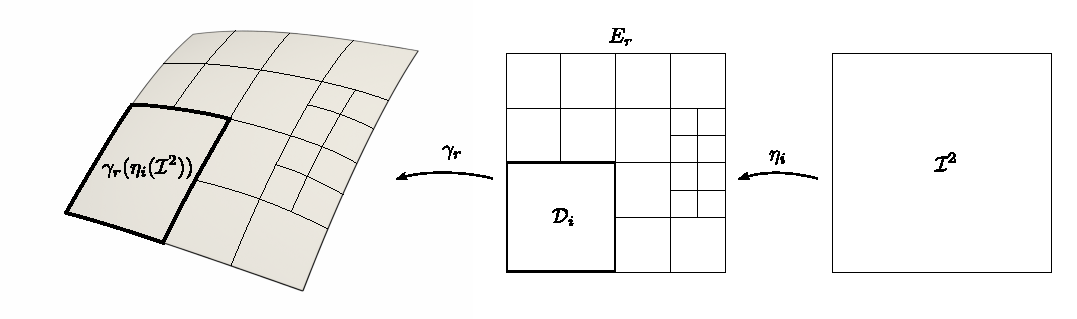
\includegraphics[width=\linewidth]{figs/quadrisection.pdf}
  \end{minipage}\hfill
%  \mcaption{fig:geometry-representation}{Patch Quadrisection}{
%      Right: the standard domain $\mathcal{I}^2$ of a single surface or quadrature patch.
%    Middle: a collection of subdomains $\mathcal{D}_i$ of $E_r$, produced by quadrisection. 
%    Each $\mathcal{D}_i$ corresponds to a map $\eta_i$ such that $\mathcal{D}_i = \eta_i(\mathcal{I}^2)$; a single $\mathcal{D}_i$ is highlighted in bold.
%    Left: the image of $E_r$ under the patch $\gamma_r$. 
%    The final image of each subdomain is outlined, with the image of $\mathcal{D}_i$ in bold.
%  }
\end{figure}
We assume that the smooth domain boundary $\Gamma$ is given by a \textit{quadrilateral mesh} consisting of quadrilateral faces $Q_r$, referred to as \textit{quads}.
Each quad is associated with a parametric domain $\I^2 =  [-1,1]^2 = E_r$, along with embeddings $\gamma_r : E_r \to \mathbb{R}^3$ for each quad such that $Q_r = \gamma_r(E_r)$.  
We assume that the quad mesh is \textit{conforming}, i.e., two non-disjoint faces either share a whole edge or a single vertex; examples of this are shown in \Cref{fig:greens-id-test-cases,fig:solver-conv-test-cases}.
We assume that no two images $\gamma_r(E_r)$ intersect, except along the shared edge or vertex.
The surface $\Gamma$ is the union of patches $\cup_r \gamma_r(E_r) = \cup_r Q_r$.
We also assume that $\Gamma$ is sufficiently smooth to recover the solution of \cref{eq:pde} up to the boundary \cite{K} and is at least $C^k$. 

To represent the surface geometry, we approximate $\Gamma$ with a collection of \emph{B\'ezier patches}, given by a linear combination of tensor-product Bernstein polynomials
\begin{equation}
    \vP_i(s,t) = \sum_{\ell =0}^n\sum_{m =0}^n \vector{a}^{(i)}_{\ell m }B_\ell^n(s)B_m^n(t),
  \label{eq:tensor-product}
\end{equation}
where  $B_\ell^n(t) = \binom{n}{\ell} t^{n-\ell}(1-t)^{\ell}$ for each $\ell$ are the $n$-th degree Bernstein polynomials, $i$ denotes the index of a patch in the collection and $\vector{a}_{\ell m}^{(i)} \in \mathbb{R}^3$.
Each patch $\vP$ is a vector function from $\I^2$ to $\mathbb{R}^3$, so $s,t\in [-1,1]$.
We will refer to this approximation of $\Gamma$ as $\hat{\Gamma}$. % and detail its construction in \cref{sec:admissible}.
%More specifically, we use a \emph{forest of quad trees of B\'ezier patches}. 

The domain $E_r$ of each embedding function $\gamma_r$ is adaptively refined using \emph{quadrisection}, i.e., splitting a square domain into four square subdomains of equal size. %This yields a quad tree of subdomains for each face of the quad mesh.
Quadrisection induces a \textit{quadtree} structure on each $E_r$. 
The root of the quadtree is the original domain $\I^2$ and each node of the tree is related by a single quadrisection of a subdomain of $E_r$. 
The leaves of the quadtree form a collection of subdomains $\mathcal{D}_i$ whose union equals $E_r$, as shown in \cref{fig:geometry-representation}-middle.
Given an indexing scheme of all $\mathcal{D}_i$'s over all $E_r$'s, we define the function $r(i)$ that maps the leaf node index $i$ to its root node index $r$ in the quadtree forest, indicating that $\mathcal{D}_i \subset E_r$. 
For each $r$, $E_r$ can have a distinct sequence of associated quadrisections and therefore a distinct quadtree structure.
We refer to the process of \textit{refinement} or \textit{refining a patch $\vP$} as the construction of such quadtrees for each $E_r$ subject to some set of criteria.

On each $\mathcal{D}_i$ at the quadtree leaves, we define a B\'ezier patch and reparametrize each patch over $\I^2$ by defining the affine map $\eta_i: \I^2 \to E_{r(i)}$ such that $\eta_i(\I^2) = \mathcal{D}_i \subseteq E_{r(i)}$.
%On each $\mathcal{D}_i$ at the quadtree leaves, we define a \emph{B\'ezier patch} given by a linear combination of  tensor-product Bernstein polynomials on $\mathcal{D}_i$:
%\begin{equation}
%    P(s,t) = \sum_{\ell =0}^n\sum_{m =0}^n \vector{a}_{\ell m }B_\ell^n(s)B_m^n(t),
%  \label{eq:tensor-product}
%\end{equation}
%where  $B_k^n(t) = \binom{n}{k} t^{n-k}(1-t)^{k}$ is $n$-th degree Bernstein polynomials.
It follows that the set of subdomains $\{ \eta_i(\I^2) \,| \,r(i) = \kappa\}$ form a cover of $E_\kappa$ and $\{ \gamma_\kappa(\eta_i(\I^2))\, | \,r(i) = \kappa\}$ likewise covers $\gamma_\kappa(E_\kappa)$.
We summarize this setup in \Cref{fig:geometry-representation}; examples of surfaces of this form can be seen in \Cref{fig:greens-id-test-cases,fig:solver-conv-test-cases,fig:torii,fig:vessel}.
%Since we have made no assumptions on the explicit form of $\gamma_r$, this approximation stage constructs a consistent surface representation that we can leverge in our algorithms in \cref{sec:admissible} without sacrificing geometric fidelity.
%At each step of quadrisection, there is a parent-child relationship formed between the subdomain and its four resulting subdomains. 
%In \Cref{fig:geometry-representation}-right, we have a single leaf of this quadtree, denoted $D_i$.

%The coefficients or \emph{control points} $\vector{a}_{\ell m}$ in \cref{eq:tensor-product} are computed to fit the B\'ezier patches to the input embeddings $\gamma_r$.
%Each patch $P_i$ in $\Pcoarse$ is reparametrized on $\I^2$ and each domain is associated with a leaf of the forest of quad trees.
%We refer to the domain of $P_i$ by $D_{i}$, noting that $D_i = \I^2$. 
%Each such domain $D_i$ corresponds to a subdomain of $E_{r(i)}$, where $r(i)$ is the index of the embedding $\gamma_{r(i)}$ from which
%$P_i$ was obtained by refinement.
%Define the  map $\eta_i: D_i \rightarrow E_{r(i)}$, which embeds the domain $D_i$ into the copy of $\I^2$ corresponding to $\gamma_{r(i)}$. 
%The set of maps $\{\eta_i \mid r(i) = k\}$ cover $\I^2$ for each embedding map $\gamma_k$.
%We summarize this setup in \cref{fig:geometry-representation}.

%In the simplest case, the input is already in B\'ezier form and no additional processing is necessary; the overall accuracy of our method is limited by therefore by the smoothness of the given polynomial surface.
%In general, $\Gamma$ can be defined by arbitrary functions. 
%The domain on which the complete approximate surface $\hat{\Gamma}$ is defined is the union of $E_{r(i)}$ identified along shared edges. 
%The complete set of B\'ezier patches defined on these domains is denoted $\Pcoarse$.

\subsection{Problem discretization \label{sec:discretization}}
We use two collections of patches in the form described above: $\Pcoarse$ and $\Pfine$.
The patches in $\Pcoarse$, called \emph{surface patches}, determine $\Gammah$ from $\Gamma$ and the set of patches $\Pfine$, called \emph{quadrature patches}, are obtained by further quadrisection of the surface patches in $\Pcoarse$.
The geometry of $\Gammah$ is not changed by this additional refinement of $\Pcoarse$, but the total number of subdomains $E_{r(i)}$ is increased.
We will detail the geometric criteria that $\Pcoarse$ and $\Pfine$ must satisfy in \cref{sec:geom_criteria}.
Discretizing $\Gammah$ with with a quadrature rule based on $\Pfine$ results in a denser sampling of $\Gammah$ than a similar discretization of $\Pcoarse$.
We will refer to $\Pcoarse$ as the \textit{coarse discretization} of $\hat{\Gamma}$ and $\Pfine$ as the \textit{upsampled} or \textit{fine discretization} of $\hat{\Gamma}$.

We index the patches in $\vP_i \in \Pcoarse$ by $i = 1,\hdots N$; we can then rewrite \cref{eq:double_layer} as a sum of integrals over surface patches:
\begin{equation}
  u(\vx) = \sum_{i=1}^N\int_{\vP_i} \frac{\partial G(\vx,\vy)}{\partial \vn(\vy)} \phi(\vy) d\vy_{\vP_i}.
  \label{eq:double_layer_patches} 
\end{equation}

%The coefficients $a_{ij}$ of $P(u,v)$, or \textit{control points}, have geometric relevance: the convex hull of the control points contains $P$, yielding a simple algorithm for computing a bounding box for a patch image.

%The control points of B\'ezier patches also admit an efficient algorithm to compute control points on subdomains of the domain of $P$ via a \emph{subdivision} \cite{F}. This fact is used in \cref{sec:adaptive_upsampling,sec:mark_near}. Subdivision is used for two purposes: obtain an accurate surface approximation with B\'ezier patches, and obtain admissible \emph{quadrature patches} from surface patches, as explained below. 

%In the case of surfaces specified by a black-box evaluator on the initial quad mesh,  we fit tensor-product B\'ezier patches to each $\gamma_i$, adaptively subdividing each original patch as necessary, until a desired absolute error in function values is achieved. In the former case, the accuracy of the solution is restricted by the accuracy of the given surface approximation. 


%Ideally, each surface patch is defined as in \cref{eq:tensor-product}; however, we do not assume that this is the case in practice.
%If surface patches are defined in another tensor-product polynomial basis or splines, one can perform a change of variables to express them in the form of \cref{eq:tensor-product}.

%An important property of the method presented in this work is that we make minimal assumptions on the input geometry definition and boundary data; the accuracy our method can achieve is ultimately bounded by their smoothness.


We discretize functions defined on $\Gammah$, such as
\cref{eq:double_layer_patches}, at $q$-node composite tensor-product
Clenshaw-Curtis quadrature points on $\I^2$ of patches in $\Pcoarse$.  
We refer to these points and weights on a single patch $\vP_i$ as $x_j$ and $w_j^{\lbl{CC}}$ respectively, for $j = 1\ldots q^2$. 
%The weights are given by $w_j = \sqrt{g_j}w_j^{\lbl{CC}}$, with $g_j$ being the determinant of the metric tensor of $\vP$ at $x_j$ and $w_j^{\lbl{CC}}$ is the Clenshaw-Curtis weight at $x_j$.
The quadrature point $\vy_{ij}$ from $\vP_i$ is defined as $\vy_{ij} = \vP_{i}(\eta_i(x_j))$. 
We assume that the boundary condition $f$ is given by a black-box evaluator on $\mathbb{R}^3$ that can be used to obtain values at $\vy_{ij}$.
For clarity, we reindex the surface points by a global index $I = 1, \hdots, q^2N$.
%For the remainder of this work, we will suppress the explicit dependence of $P_i$ on the parametrization $\eta_i$. \note[MJM]{check that this is needed}
We discretize the double layer integral \cref{eq:double_layer_patches} on $\Pcoarse$ to approximate the solution $u(\vx)$:
%\begin{equation}
%  \left(\frac{1}{2}I + \hat{D} + \hat{M}\right)[\phi](\vy_\ell) = f(\vy_\ell), \quad \ell=1,\hdots N
%  \label{eq:int-eq-disc}
%\end{equation}
%with the discretized double layer operator $\hat{D}[\phi](\vy)$ defined as 
\begin{equation}
    u(\vx,\Pcoarse) \approx \hat{u}(\vx,\Pcoarse) = \sum_{i=1}^N\sum_{j=1}^{q^2} \frac{\partial G(\vx,\vy_{ij})}{\partial \vn(\vy_{ij})} \phi_{ij} \sqrt{g_{ij}}w_j^{\lbl{CC}} 
    = \sum_{I=1}^{q^2N}\frac{\partial G(\vx,\vy_I)}{\partial \vn(\vy_I)} \phi_I \hat{w}_I
  \label{eq:double_layer_disc}
  %\label{eq:double_layer_disc}
\end{equation}
with $g_{ij}$ being the determinant of the metric tensor of $\vP_i$ at $x_j$ and $\hat{w}_{i\cdot q^2+j} = \sqrt{g_{ij}}w_{j}^{\lbl{CC}}$.
In other words, $\hat{u}(\vx, \Pcoarse) = \hat{D}[\phi](\vx)$, where $\hat{D}[\phi](\vx) \approx D[\phi](\vx)$.

We can also discretize functions with tensor-product Clenshaw-Curtis nodes on the domains of patches in $\Pfine$.
The values of functions on $\Pfine$ are \emph{interpolated} from their values on the quadrature nodes of $\Pcoarse$ rather than being computed directly on $\Pfine$.
We call this interpolation from $\Pcoarse$ to $\Pfine$ \textit{upsampling}.
We denote the quadrature nodes and weights on $\Pfine$ by $\tilde{x}_j$ and $\tilde{w}_j$ with a similar global index $J$ and refer to them as the \textit{upsampled} nodes and weights.
Identical formulas are used for computing quadrature on $\Pfine$ with the nodes and weights $\tilde{x}_j$, $\tilde{w}_j$ on $\Pfine$, denoted $u(\vx,\Pfine)$ and $\hat{u}(\vx,\Pfine)$, repsectively.

In the next section, we describe the algorithm to compute an accurate approximation to the singular/near-singular double-layer integral in \cref{eq:double_layer}, using a quadrature rule for smooth functions (\cref{eq:double_layer_disc}) as a building block. 
This algorithm allows us to compute the matrix-vector products $A\phi$, for a vector of values $\phi$ defined at the quadrature points $\vy_I$, where $A$ is the discrete operator obtained from the left-hand side of \cref{eq:int-eq} after approximating $D[\phi](\vy)$ with the singular integration scheme.
As a result, we can solve the linear system using \gmres, which only requires a matrix-vector product 
\begin{equation}
  A\phi = f,
  \label{eq:linear_system}
\end{equation}
where $f$ is the boundary condition sampled at the points $\vy_I$. The evaluation of these integrals is accelerated in a standard manner using the fast multipole method (\fmm)\cite{MB,ying2004kernel,greengard1987fast}.
%The index in the sum in \cref{eq:double_layer_disc} ranges over all quadrature nodes on all quadrature patches. 
%This results in a linear system for the values of the density at the quadrature nodes on the boundary:
%\begin{equation}
%  A\phi = f, \quad A_{ij} = \frac{\delta_{ij}}{2} + \frac{\partial G(\vy_i, \vy_j)}{\partial \vn(\vy_j)} + M_{ij},
%  \label{eq:linear_system}
%\end{equation}
%where $\delta_{ij}$ is the Kronecker delta. \note[DZ]{need to define $M_{ij}$.} 
%$A$ is dense, but we can apply $A$ to a vector in linear time,  due to the low-rank structure of off-diagonal blocks, using fast-multipole method (\fmm). The integral equation is well-conditioned and 
%in conjunction with GMRES to solve \cref{eq:linear_system}.
%However, the entries of this system matrix become singular as they approach the diagonal; singular quadrature rules are need to compute these values accurately.


